\documentclass[10pt]{beamer}
\usetheme{Antibes}
\usepackage[utf8]{vietnam}
\usepackage{ragged2e}
\usepackage{graphicx}
% \usepackage[dvips]{color}
% coding styles  %%%%%%%%%% font for code terminal
% \setbeamercovered{transparent}
\usepackage{listings}
\usepackage{color}
\definecolor{lightgray}{rgb}{.9,.9,.9}
\definecolor{darkgray}{rgb}{.4,.4,.4}
\definecolor{purple}{rgb}{0.65, 0.12, 0.82}
\definecolor{pink}{rgb}{0.9, 0.25, 0.8}

\definecolor{maroon}{cmyk}{0, 0.87, 0.68, 0.32}
\definecolor{halfgray}{gray}{0.55}
\definecolor{ipython_frame}{RGB}{207, 207, 207}
\definecolor{ipython_bg}{RGB}{247, 247, 247}
\definecolor{ipython_red}{RGB}{186, 33, 33}
\definecolor{ipython_green}{RGB}{0, 128, 0}
\definecolor{ipython_cyan}{RGB}{64, 128, 128}
\definecolor{ipython_purple}{RGB}{170, 34, 255}

\lstset{
    breaklines=true,
    extendedchars=true,
    literate=
    {á}{{\'a}}1 {é}{{\'e}}1 {í}{{\'i}}1 {ó}{{\'o}}1 {ú}{{\'u}}1
    {Á}{{\'A}}1 {É}{{\'E}}1 {Í}{{\'I}}1 {Ó}{{\'O}}1 {Ú}{{\'U}}1
    {à}{{\`a}}1 {è}{{\`e}}1 {ì}{{\`i}}1 {ò}{{\`o}}1 {ù}{{\`u}}1
    {À}{{\`A}}1 {È}{{\'E}}1 {Ì}{{\`I}}1 {Ò}{{\`O}}1 {Ù}{{\`U}}1
    {ä}{{\"a}}1 {ë}{{\"e}}1 {ï}{{\"i}}1 {ö}{{\"o}}1 {ü}{{\"u}}1
    {Ä}{{\"A}}1 {Ë}{{\"E}}1 {Ï}{{\"I}}1 {Ö}{{\"O}}1 {Ü}{{\"U}}1
    {â}{{\^a}}1 {ê}{{\^e}}1 {î}{{\^i}}1 {ô}{{\^o}}1 {û}{{\^u}}1
    {Â}{{\^A}}1 {Ê}{{\^E}}1 {Î}{{\^I}}1 {Ô}{{\^O}}1 {Û}{{\^U}}1
    {œ}{{\oe}}1 {Œ}{{\OE}}1 {æ}{{\ae}}1 {Æ}{{\AE}}1 {ß}{{\ss}}1
    {ç}{{\c c}}1 {Ç}{{\c C}}1 {ø}{{\o}}1 {å}{{\r a}}1 {Å}{{\r A}}1
    {€}{{\EUR}}1 {£}{{\pounds}}1
}

\lstdefinelanguage{Python}{
    morekeywords={access,and,break,class,continue,def,del,elif,else,except,exec,finally,for,from,global,if,import,in,is,lambda,not,or,pass,print,raise,return,try,while},
    morekeywords=[2]{abs,all,any,basestring,bool,bytearray,callable,chr,classmethod,cmp,compile,complex,delattr,dict,dir,divmod,enumerate,eval,execfile,file,filter,float,format,frozenset,getattr,globals,hasattr,hash,help,hex,id,input,int,isinstance,issubclass,iter,len,list,locals,long,map,max,memoryview,min,next,object,oct,open,ord,pow,property,range,raw_input,reduce,reload,repr,reversed,round,set,setattr,slice,sorted,staticmethod,str,sum,super,tuple,type,unichr,unicode,vars,xrange,zip,apply,buffer,coerce,intern},
    sensitive=true,
    morecomment=[l]\#,
    morestring=[b]',
    morestring=[b]",
    morestring=[s]{'''}{'''},
    morestring=[s]{"""}{"""},
    morestring=[s]{r'}{'},
    morestring=[s]{r"}{"},
    morestring=[s]{r'''}{'''},
    morestring=[s]{r"""}{"""},
    morestring=[s]{u'}{'},
    morestring=[s]{u"}{"},
    morestring=[s]{u'''}{'''},
    morestring=[s]{u"""}{"""},
    % {replace}{replacement}{lenght of replace}
    % *{-}{-}{1} will not replace in comments and so on
    literate=
    {á}{{\'a}}1 {é}{{\'e}}1 {í}{{\'i}}1 {ó}{{\'o}}1 {ú}{{\'u}}1
    {Á}{{\'A}}1 {É}{{\'E}}1 {Í}{{\'I}}1 {Ó}{{\'O}}1 {Ú}{{\'U}}1
    {à}{{\`a}}1 {è}{{\`e}}1 {ì}{{\`i}}1 {ò}{{\`o}}1 {ù}{{\`u}}1
    {À}{{\`A}}1 {È}{{\'E}}1 {Ì}{{\`I}}1 {Ò}{{\`O}}1 {Ù}{{\`U}}1
    {ä}{{\"a}}1 {ë}{{\"e}}1 {ï}{{\"i}}1 {ö}{{\"o}}1 {ü}{{\"u}}1
    {Ä}{{\"A}}1 {Ë}{{\"E}}1 {Ï}{{\"I}}1 {Ö}{{\"O}}1 {Ü}{{\"U}}1
    {â}{{\^a}}1 {ê}{{\^e}}1 {î}{{\^i}}1 {ô}{{\^o}}1 {û}{{\^u}}1
    {Â}{{\^A}}1 {Ê}{{\^E}}1 {Î}{{\^I}}1 {Ô}{{\^O}}1 {Û}{{\^U}}1
    {œ}{{\oe}}1 {Œ}{{\OE}}1 {æ}{{\ae}}1 {Æ}{{\AE}}1 {ß}{{\ss}}1
    {ç}{{\c c}}1 {Ç}{{\c C}}1 {ø}{{\o}}1 {å}{{\r a}}1 {Å}{{\r A}}1
    {€}{{\EUR}}1 {£}{{\pounds}}1
    %
    {^}{{{\color{ipython_purple}\^{}}}}1
    {=}{{{\color{ipython_purple}=}}}1
    %
    {+}{{{\color{ipython_purple}+}}}1
    {*}{{{\color{ipython_purple}$^\ast$}}}1
    {/}{{{\color{ipython_purple}/}}}1
    %
    {+=}{{{+=}}}1
    {-=}{{{-=}}}1
    {*=}{{{$^\ast$=}}}1
    {/=}{{{/=}}}1,
    literate=
    *{-}{{{\color{ipython_purple}-}}}1
     {?}{{{\color{ipython_purple}?}}}1,
    %
    identifierstyle=\color{black}\ttfamily,
    commentstyle=\color{ipython_cyan}\ttfamily,
    stringstyle=\color{ipython_red}\ttfamily,
    keepspaces=true,
    showspaces=false,
    showstringspaces=false,
    rulecolor=\color{ipython_frame},
    frame=single,
    frameround={t}{t}{t}{t},
    framexleftmargin=6mm,
    numbers=left,
    numberstyle=\tiny\color{halfgray},
    backgroundcolor=\color{ipython_bg},
    % extendedchars=true,
    basicstyle=\scriptsize,
    keywordstyle=\color{ipython_green}\ttfamily,
}
\lstdefinelanguage{JavaScript}{
  keywords={typeof, new, true, false, catch, function, return, null, catch, switch, var, if, in, while, do, else, case, break},
  keywordstyle=\color{blue}\bfseries,
  ndkeywords={var, class, export, boolean, throw, implements, import, this},
  ndkeywordstyle=\color{pink}\bfseries,
  identifierstyle=\color{black},
  sensitive=false,
  comment=[l]{//},
  morecomment=[s]{/*}{*/},
  commentstyle=\color{purple}\ttfamily,
  stringstyle=\color{red}\ttfamily,
  morestring=[b]',
  morestring=[b]"
}
\lstdefinelanguage{VueJS}{
  keywords={template, div, h1, h2, h3, h4, h5, h6, script, style, new},
  keywordstyle=\color{blue}\bfseries,
  ndkeywords={var, class, export, boolean, throw, implements, import, default},
  ndkeywordstyle=\color{pink}\bfseries,
  emph={Vue},
  emphstyle=\color{ipython_green},
  identifierstyle=\color{black},
  sensitive=false,
  comment=[l]{//},
  morecomment=[s]{/*}{*/},
  commentstyle=\color{ipython_green}\ttfamily,
  stringstyle=\color{red}\ttfamily,
}

\lstset{
   backgroundcolor=\color{lightgray},
   extendedchars=true,
   basicstyle=\footnotesize\ttfamily,
   showstringspaces=false,
   showspaces=false,
   numbers=left,
   numberstyle=\footnotesize,
   numbersep=9pt,
   tabsize=2,
   breaklines=true,
   showtabs=false,
   captionpos=b
}


% end coding styles

\graphicspath{{./img/}}

\title{FTech Training}
\subtitle{Using Beamer}
\author{Luc Nguyen}
\institute{HUST}
\date{\today}
\usetheme{Boadilla}


\begin{document}
\begin{frame}
    \frametitle{\textbf{DOCCANO WITH VUEJS AND WEBPACK}}
    \begin{minipage}{0.43\textwidth}
        \Large{\textbf{OUTLINE}}  \\
        \begin{enumerate}
            \item VueJS
            % \begin{itemize}
                % \item Basic concepts
                % \item Real-world Vue
                % \item Vue frameworks
                % \item Miscellaneous
            % \end{itemize}
            \item Webpack
            \item Doccano
            \item References %If you understand your data, you should tailor made augmentation approach it
        \end{enumerate}
    \end{minipage}
    \begin{minipage}{0.55\textwidth}
        
\includegraphics[scale=0.2]{vue.png}
        
\includegraphics[scale=0.1]{webpack.png}
        
\includegraphics[scale=0.35]{doccano.png}
    \end{minipage}
\end{frame}
\begin{frame}[fragile]
    \frametitle{\textbf{VUEJS}}
    \framesubtitle{\textbf{Basic concepts}}
    \begin{itemize}
        \item Unlike other monolithic frameworks, Vue is designed from the ground up to be incrementally adoptable
        % \pause
        \item Vue instance
        \begin{itemize}
            \item Every Vue application starts by creating a new Vue instance with the Vue function:
            \begin{lstlisting}[language=VueJS] 
    var vm = new Vue({
        // options
    })
            \end{lstlisting}
            % \item Lifecycle hooks and Lifecycle diagram
        \end{itemize}
    \end{itemize}
\end{frame}
\begin{frame}
    \frametitle{\textbf{VUEJS}}
    \framesubtitle{\textbf{Basic concepts}}
    Lifecycle hooks and Lifecycle diagram 
    {\centering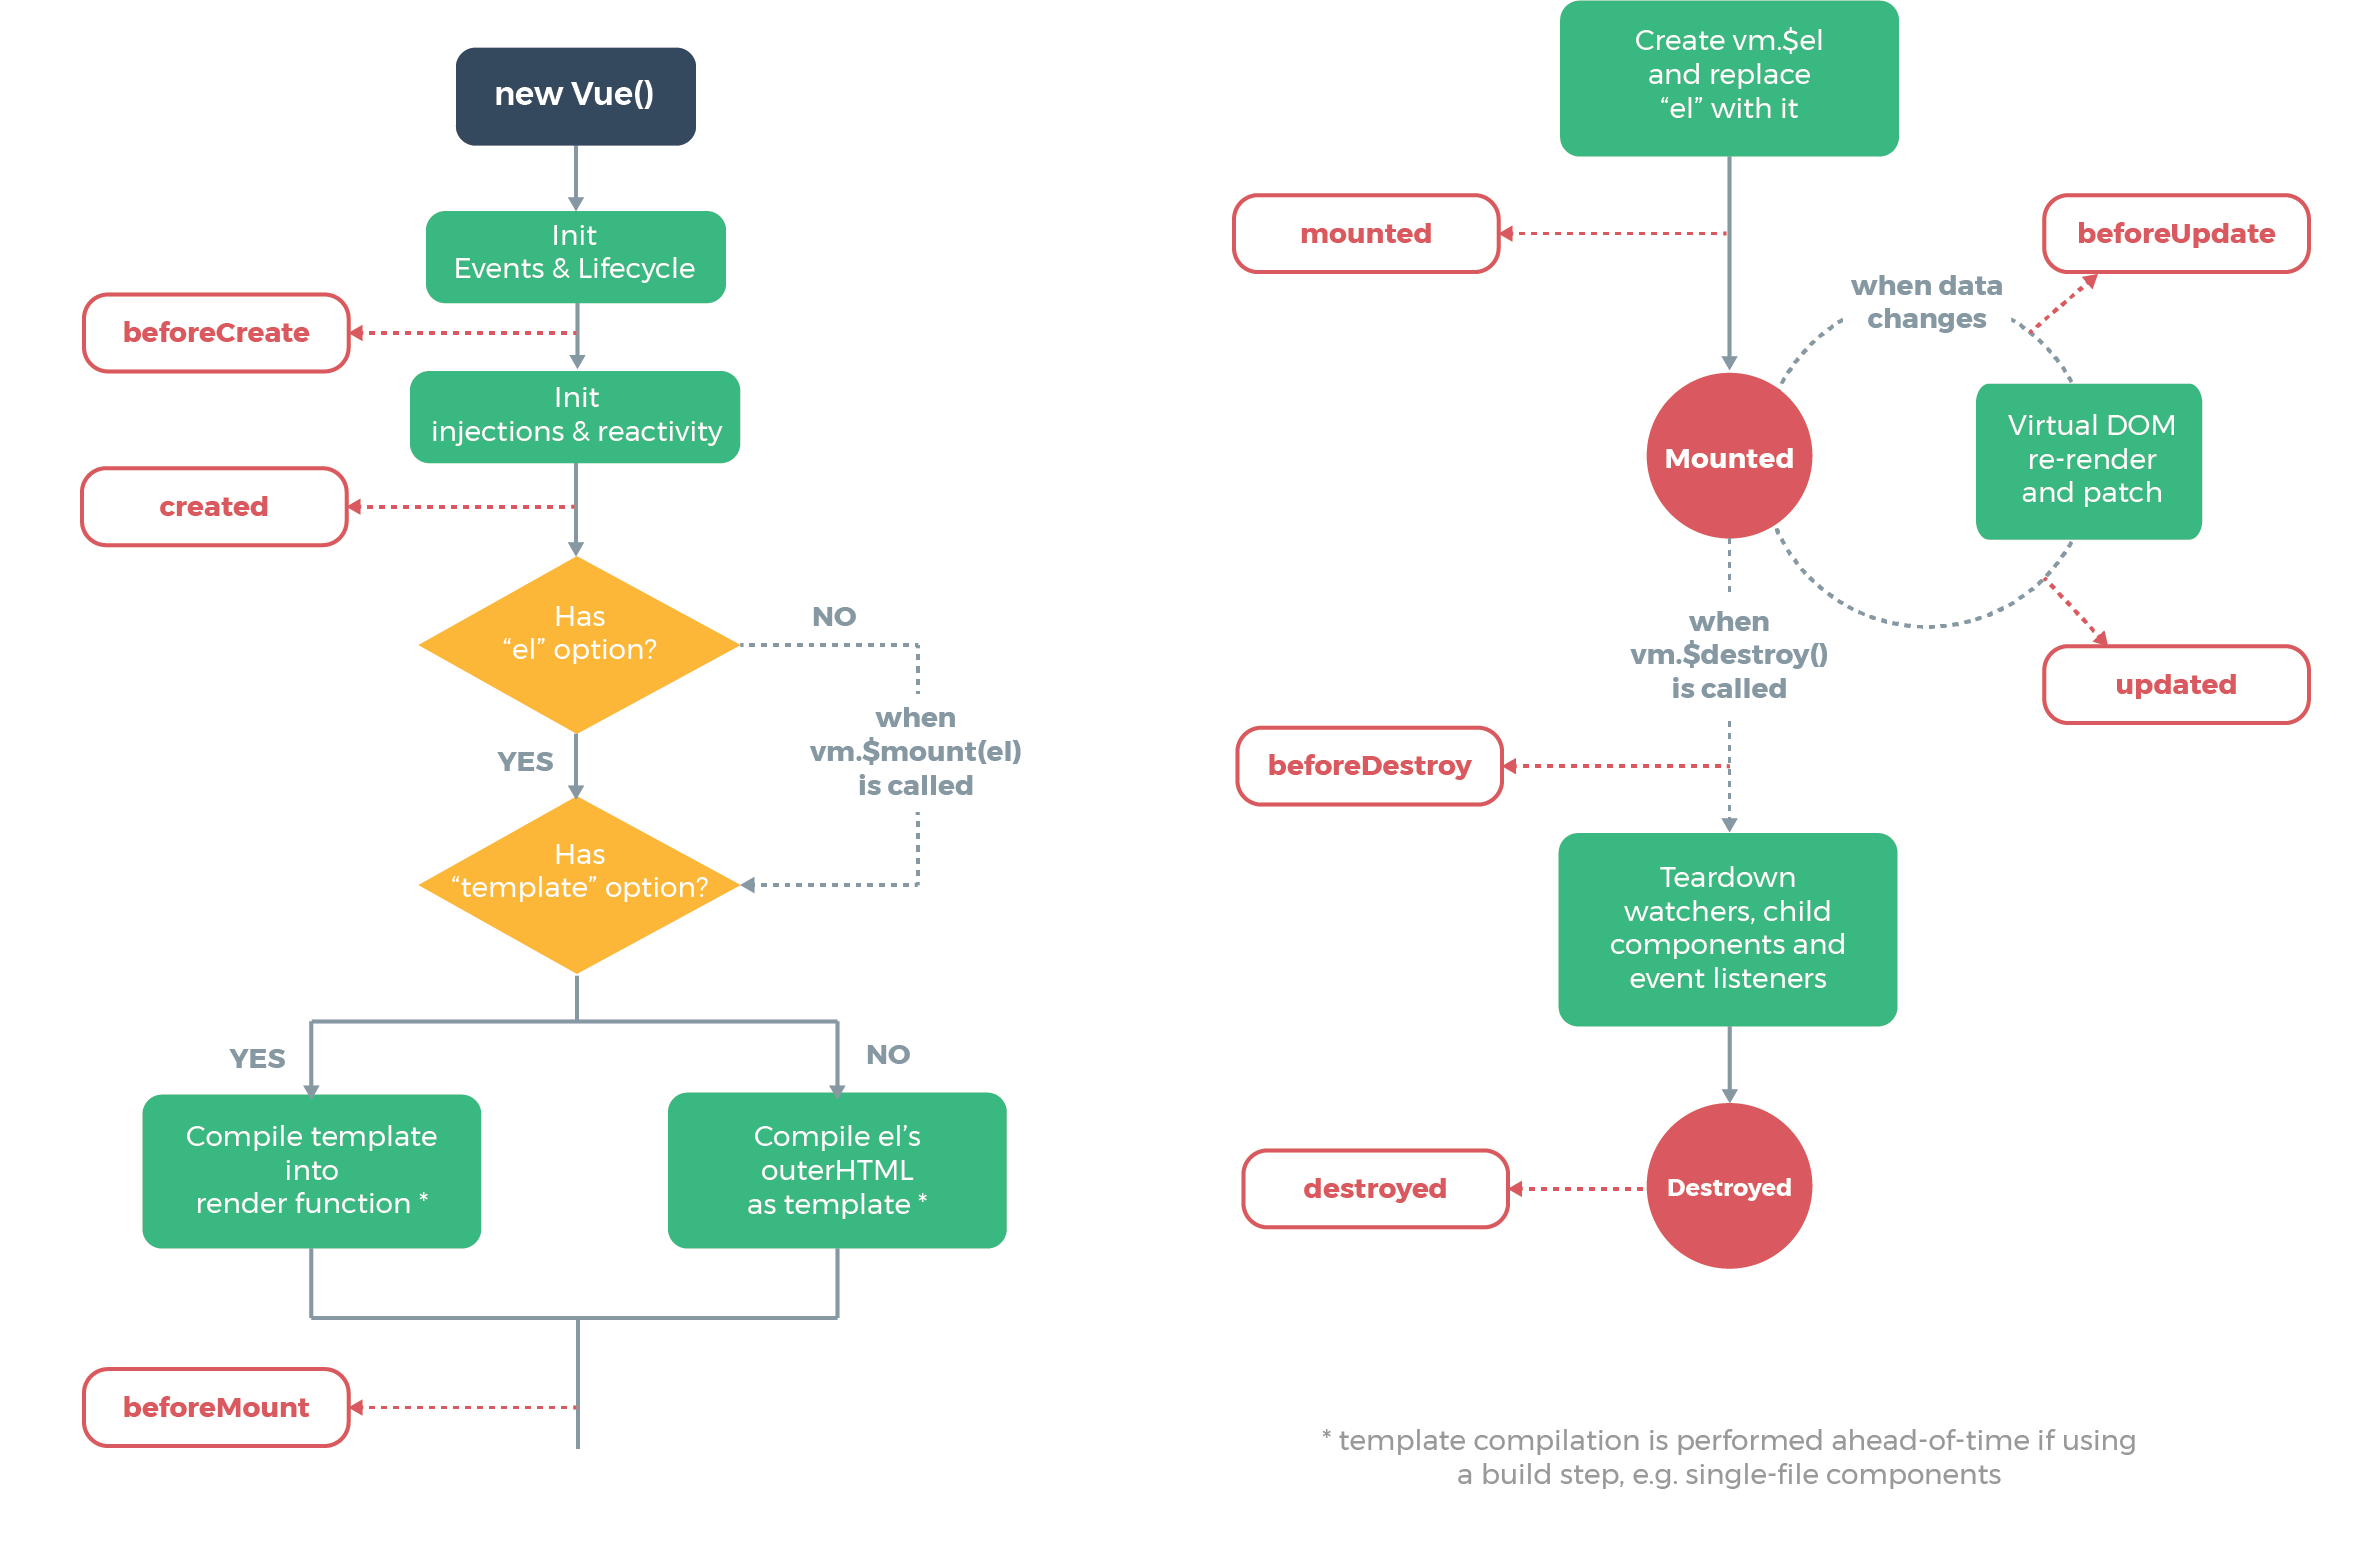
\includegraphics[scale=0.14]{vue_lifecycle.png}\par}
\end{frame}
\begin{frame}[fragile]
    \frametitle{\textbf{VUEJS}}
    \framesubtitle{\textbf{Basic concepts}}
    \begin{itemize}
        \item Vue components: reusable Vue instances with a name.
        % \pause
        \begin{minipage}{0.5\textwidth}
            \begin{lstlisting}[language=VueJS, caption=HelloWorld.vue]
<template>
<div class="hello">`
<h1> This is HelloWorldd </h1>
</div>
</template>
<script>
export default {
    name: 'HelloWorld',
}
</script>
            \end{lstlisting}
        \end{minipage}
        \hspace{0.1\textwidth}
        % \pause
        \begin{minipage}{0.3\textwidth}
            \begin{lstlisting}[language=VueJS, caption=App.vue]
<template>
  <div id="app">
    <HelloWorld/>
    <HelloWorld/>
    <HelloWorld/>
  </div>
</template>
            \end{lstlisting}
        \vspace{1cm}
        % \pause
        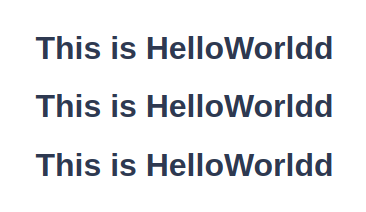
\includegraphics[scale=0.3]{helloworld.png}
        \end{minipage}
    \end{itemize}
\end{frame}
\begin{frame}
    \frametitle{\textbf{VUEJS}}
    \framesubtitle{\textbf{Basic concepts}}
    \begin{itemize}
        \item Single-page applications : a web application or web site that interacts
             with the user by dynamically rewriting the current page rather than loading
             entire new pages from a server.
             \begin{itemize}
                 \item \href{https://router.vuejs.org/}{\underline{Vue Router}} : tool for building SPAs maintained by the Vue team.
             \end{itemize}
        % \pause
        \item State management : 
        \begin{itemize}
            \item \href{https://vuex.vuejs.org/}{\underline{Vuex}} : tool for managing global state and components by the Vue team.
            \begin{itemize}
                \item State
                \item Getters
                \item Mutations
                \item Actions
            \end{itemize}
        \end{itemize}
    \end{itemize}
\end{frame}
\begin{frame}
    \frametitle{\textbf{VUEJS}}
    \framesubtitle{\textbf{Real-world Vue}}
    \begin{itemize}
        \item Project scaffolding: \href{https://cli.vuejs.org/}{\underline{Vue CLI}} initialize a Vue project in minutes. 
        % \pause
        \item Data-driven user interfaces: the data will often be sourced from a secure API.
        % \pause
        \item Testing: \href{https://vue-test-utils.vuejs.org/}{\underline{Vue Test Utils}} allows to create and run tests on isolated Vue components.
    \end{itemize}
\end{frame}
\begin{frame}
    \frametitle{\textbf{VUEJS}}
    \framesubtitle{\textbf{Vue-based frameworks}}
    % \pause
    \begin{itemize}
        \item \href{https://nuxtjs.org/}{\underline{Nuxt.js}}: a framework provide  a high-performance Vue app with component-based routing, server-side rendering, code splitting.
        % \pause
        \item \href{https://vuetifyjs.com/en/}{\underline{Vuetify}}: quickly build Vue apps with Material Design layout and styling, plus widgets like modals, alerts, navbars, pagination etc.
        % \pause
        \item \href{https://nativescript-vue.org/}{\underline{NativeScript-Vue}}: an open source plugin which allows you to use Vue.js to craft your mobile application.
    \end{itemize}
\end{frame}
\begin{frame}
    \frametitle{\textbf{WEBPACK}}
    \framesubtitle{\textbf{Basic concepts}}
    % \pause
    \begin{definition}[Webpack]
        At its core, \href{https://webpack.js.org/}{\underline{webpack}} is a static module bundler for modern JavaScript applications.
    \end{definition}
    % \pause
    \begin{itemize}
        \item If your code is written across different modules, Webpack can "build" these into one single file that is readable by a browser.
    \end{itemize}
    {\centering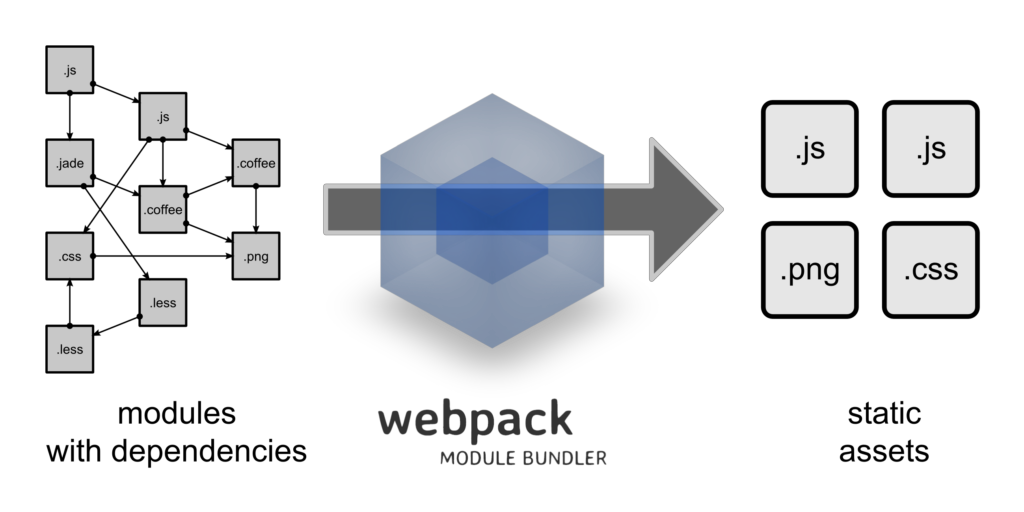
\includegraphics[scale=0.25]{webpack_overview.png}\par}
\end{frame}
\begin{frame}
    \frametitle{\textbf{WEBPACK}}
    \framesubtitle{\textbf{Webpack 5 structure}}
    \large{\textbf{Basic parameters:}}
    \begin{itemize}
        % \pause
        \item Entry points: indicates which module webpack should use to begin building out its internal dependency graph.
        % \pause
        \item Output: where to emit the bundles it creates and how to name these files.
        % \pause
        \item Loaders: process other types of files and convert them into valid modules.
        % \pause
        \item Plugins: perform a wider range of tasks like bundle optimization, asset management and injection of environment variables.
        % \pause
        \item Mode: tells webpack to use its built-in optimizations accordingly.
        \begin{itemize}
            \item 'development', 'production', 'none'
        \end{itemize} 
        % \pause
        \item Other parameters: DevTool, Resolve, Watch, .... 
    \end{itemize}
\end{frame}
\begin{frame}
    \frametitle{\textbf{DOCCANO}}
    \framesubtitle{\textbf{Basic concepts}}
    % \pause
    \begin{definition}[Doccano]
        \href{https://github.com/doccano/doccano/}{\underline{Doccano}} is an open source text annotation tool for humans.
    \end{definition}
    % \pause
    {\centering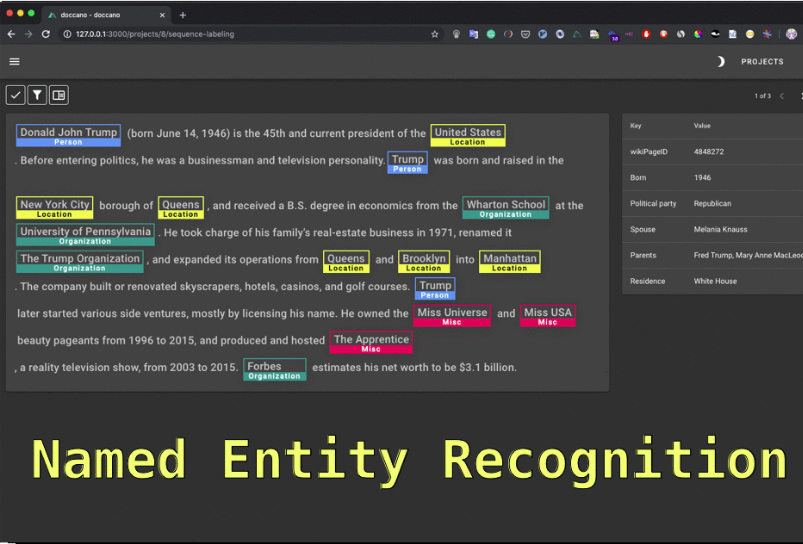
\includegraphics[scale=0.28]{doc_NER.png}\par}
\end{frame}
\begin{frame}[fragile]
    \frametitle{\textbf{DOCCANO}}
    \framesubtitle{\textbf{Some features}}
    % \large{\textbf{Steps:}}
    \begin{enumerate}
        % \pause
        \item Sentiment analysis
        % \pause
        \item Named Entity Recognition
        % \pause
        \item Translation
    \end{enumerate}
\end{frame}
\begin{frame}
    \frametitle{\textbf{DOCCANO}}
    \framesubtitle{\textbf{Basic concepts}}
    \large{\textbf{Some properties:}}
    % \pause
    \begin{itemize}
        \item Single microservice application.
        % \pause
        \item Use VueJS framework to build front-end.
        % \pause
        \item Use webpack to bundle all assets.
    \end{itemize}
\end{frame}
\begin{frame}[fragile]
    \frametitle{\textbf{DOCCANO}}
    \framesubtitle{\textbf{How to start}}
    \large{\textbf{Requirements:}}
    \begin{itemize}
        % \pause
        \item Python
        % \pause
        \item NodeJS
        \begin{lstlisting}[language=Python]
    sudo apt install nodejs
        \end{lstlisting}
        % \pause
        \item Node package manager
        \begin{lstlisting}[language=Python]
    npm install npm@latest -g
        \end{lstlisting}
        % \pause
        \item Clone doccano: 
        \begin{lstlisting}[language=Python]
    git clone https://github.com/chakki-works/doccano.git
        \end{lstlisting}
    \end{itemize}
\end{frame}
\begin{frame}[fragile]
    \frametitle{\textbf{DOCCANO}}
    \framesubtitle{\textbf{How to start}}
    \large{\textbf{Steps:}}
    \begin{enumerate}
        % \pause
        \item Create an environment : 
        \begin{lstlisting}[language=Python]
    cd doccano
    virtualenv venv
    source venv/bin/activate    # activate the environment
        \end{lstlisting}
        % \pause
        \item Install required packages :
        \begin{lstlisting}[language=Python]
    <venv> pip install -r requirements.txt # not easy
        \end{lstlisting}
    \end{enumerate}
\end{frame}
\begin{frame}[fragile]
    \frametitle{\textbf{DOCCANO}}
    \framesubtitle{\textbf{How to start}}
    \large{\textbf{Steps:}}
    \begin{enumerate}
        \setcounter{enumi}{2}
        \item Build front-end library : 
        \begin{lstlisting}[language=Python]
    <venv> cd app/server
    <venv> npm install 
        \end{lstlisting}
        % \pause
        \item Build front-end source code : 
        \begin{lstlisting}[language=Python]
    <venv> npm run build
        \end{lstlisting}
        % \pause
        \item Initialize and run doccano : 
        \begin{lstlisting}[language=Python]
    <venv> python manage.py migrate
    <venv> python manage.py runserver
        \end{lstlisting}
    \end{enumerate}
\end{frame}
\begin{frame}
    \frametitle{\textbf{REFERENCES}}
    \begin{enumerate}
        \item https://vuejsdevelopers.com/2018/12/04/vue-js-2019-knowledge-map/ 
        \item https://vuejs.org/ 
        \item https://router.vuejs.org/ 
        \item https://vuex.vuejs.org/
        \item https://webpack.js.org/ 
        \item https://vuetifyjs.com/en/
        \item https://vue-test-utils.vuejs.org/
        \item https://github.com/doccano/doccano/ 
    \end{enumerate}
\end{frame}
\end{document}